\subsection{Resultados obtenidos por el prototipo a 10.00 C}

\begin{figure}[H]
	\centering
	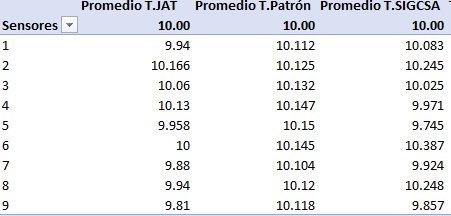
\includegraphics[width=0.5\linewidth]{resultados5.png}
	\caption{Tabla de Promedios de Temperaturas de prototipo y termómetros a 10.00 C}
\end{figure}

\par \noindent 
Los resultados obtenidos por las calibraciones, ver Anexo 4 , son utilizados para calcular la temperatura promedio del termómetro patrón, los nueve termómetros de campo de SIGCSA y los sensores de temperatura del prototipo, ver figura 4.5 y con estos valores podemos realizar la siguiente gráfica:

\begin{figure}[H]
	\centering
	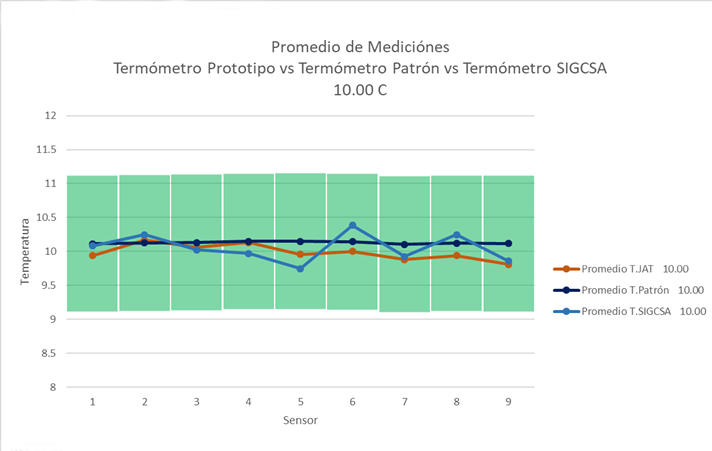
\includegraphics[width=0.6\linewidth]{resultados6.png}
	\caption{Grafico de Promedios de Temperaturas de prototipo y termómetros a 10.00 C}
\end{figure}

\par \noindent
Nuevamente tanto el prototipo como los termómetros de campo de SIGCSA se encuentran en el rango de aceptación de la compañía. Sin embargo si comparamos la figura 4.2 y la 4.6 podemos observar que a medida que la temperatura va subiendo los termómetros de campo de SIGCSA comienzan a perder exactitud con respecto al termómetro patrón. El más pronunciado de todos es el termómetro de campo numero 5, el cual se encontraba muy cerca del termómetro patrón en -10.00 grados Celsius pero ahora se alejado considerablemente de la medición del termómetro patrón. Ahora seguimos con los resultados obtenidos a 30.00 grados Celsius.
